\chapter{Experiment}
\label{sec:experiment}

\begin{itemize}
  \item Cameras and how we used them
  \item Setup check (is the setup correct?)
  \item The recording process
  \item What Exercise was chosen and why
  \item Data size (not that important but still good to give perspective)
  \item Evaluation process evaluation, how many recordings had to be discarded, how many frames were invalid, and so on
  \item How many seconds and frames were recorded in total
  \item How much data had to be discarded due to missing ground truth
  \item How much data was used for training and how much for testing
\end{itemize}

\section{Camera Setup}

The Realsense camera has an accelerometer. We know the target angle and current orientation. We can use this to fix the camera accordingly.

\begin{figure}
  \centering
  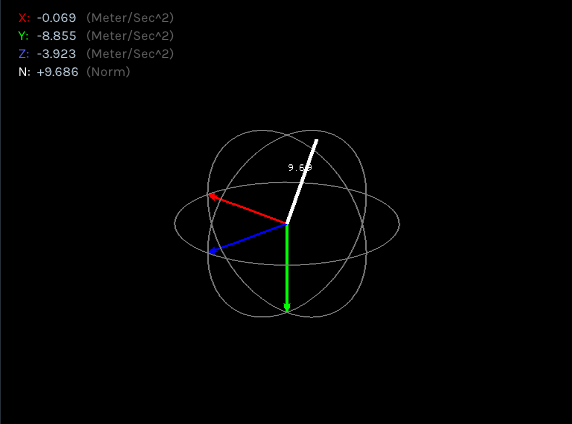
\includegraphics[width=0.5\textwidth]{figures/FESD/accelerometer.png}
  \caption{Accelerometer data from the Realsense camera used to set up the camera.}
  \label{fig:accellerometer}
\end{figure}

$$\dfrac{y}{x+y+z} * 90^{\circ} = Angle in degree $$
E.g.:
$$Angle = 70 \Rightarrow \dfrac{y}{x+y+z} * 90^{\circ} = 70^{\circ} where x = 0 \Rightarrow \dfrac{y}{y+z} = \dfrac{70}{90} $$